%!TEX root = ../thesis.tex

\section{背景}
近年,機械学習を用いた自律移動に関しての研究が盛んに行われている.本研究室でも,機械学習を用いた画像に基づく人追従行動の生成に関する研究を行ってきた.

パシンら\cite{pasin1}\cite{pasin2}\cite{pasin3}は,引き紐を利用して画像に基づく人追従行動を生成する手法を提案している.これは,深層強化学習\cite{hado}を用いており,引き紐に取り付けられたポテンショメータでリンクの角度を取得し,それに応じた報酬をエージェント(ロボット)に与えることで,画像に基づいて人追従する行動を生成できることを示した.\figref{Fig:pasin_system}にシステムの概要を示す.入力は画像で,出力を直進,左旋回,右旋回の3つとしている.

  \begin{figure}[h]
    \centering
    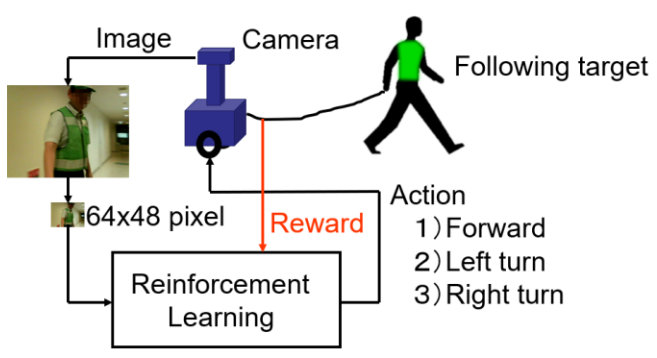
\includegraphics[keepaspectratio, scale=0.45] {images/pasin_system.png}
    \caption{Proposed method \cite{pasin1}}
    \label{Fig:pasin_system}
  \end{figure}

岡田ら\cite{okada}はこれらの技術を応用し,カメラ画像に基づく人追従行動を獲得している.ここでの教師信号はカメラ画像とルールベース制御器の出力である.

  \begin{figure}[h]
    \centering
    \begin{minipage}[c]{100mm} 
        \centering
        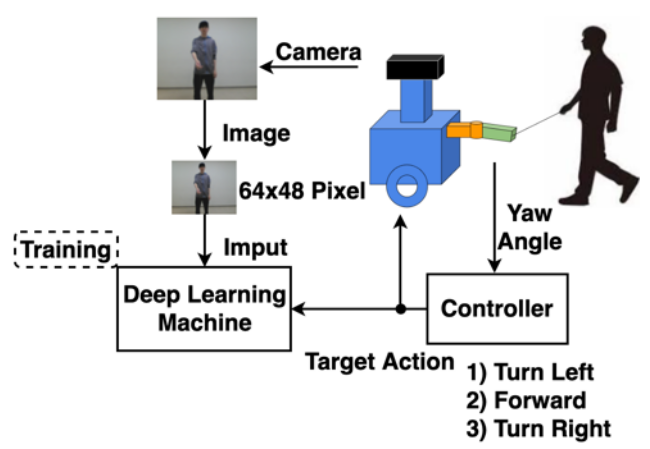
\includegraphics[width=100mm]{images/okada_learning_phase_system.png}
        \subcaption{Learning phase}
    \end{minipage} \\
    \vspace{1em} % 画像とキャプションの間にスペースを追加
    \begin{minipage}[c]{100mm} 
        \centering
        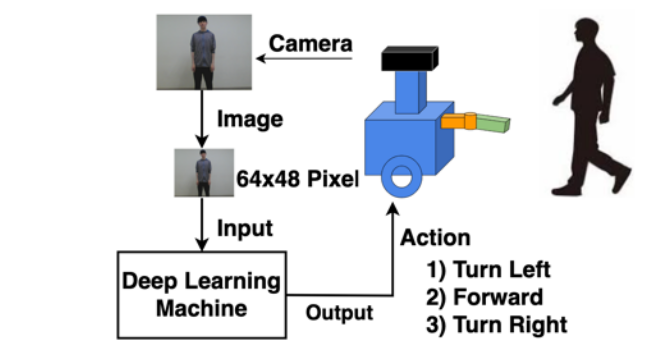
\includegraphics[width=100mm]{images/okada_following_phase_system.png}
        \subcaption{Following phase}
    \end{minipage}
    \caption{The proposed method for learning of the person-following behavior\cite{okada}}
    \label{Fig:okada_system}
  \end{figure}
% \subsection{etc...}
% \subsubsection{etc...}

\newpage
